% Print
\documentclass[DIV=15,headinclude=true]{scrartcl}

%Packages, die für die deutsche Sprache erforderlich sind
\usepackage[utf8]{inputenc}
\usepackage[T1]{fontenc}
\usepackage{lmodern}
\usepackage[ngerman]{babel}
\usepackage{csquotes}

%Packages für Graphik
\usepackage[]{graphicx}
\graphicspath{{figures/}}

%BibLaTex
\usepackage[backend=biber]{biblatex}
\addbibresource{literature/bibliography.bib} 

%Package, damit Bibtex-URL klappt
\usepackage[pdfusetitle]{hyperref}
\usepackage{url}

%Noch schönere Typographie
\usepackage{microtype}

%Kästen
\usepackage{framed}

%%%%% BEGINN KOPF- UND FUẞZEILE %%%%%
\usepackage[headsepline,footsepline]{scrlayer-scrpage}
\usepackage{graphicx}
\pagestyle{scrheadings}
\ohead{\includegraphics[height=1cm]{figures/bluemarble}}
\chead{\headmark}
\automark{section}
%\ihead{\includegraphics[height=1cm]{bluemarble.jpg}}
\ifoot{\csname @title\endcsname}\cfoot{\pagemark}
\ofoot{\today}
%%%%% ENDE KOPF- UND FUẞZEILE %%%%%

\begin{document}
%%%%% BEGINN TITEL %%%%%
\title{Präsentation in EnWiNaP}
\subtitle{Präzisierung der Anforderungen}
\author{EnWiNaP-Team}
\maketitle
%%%%% ENDE TITEL %%%%%

%%%%% BEGINN FRONT MATTER %%%%%
%\tableofcontents
%%%%% ENDE FRONT MATTER %%%%%


%%%%% BEGINN INHALT %%%%%
\section*{Editorial}

Präsentationen an einer Technischen Universität laufen in der Regel so
ab: Viele Gruppen präsentieren mehr oder weniger denselben Inhalt, mehr
oder weniger monoton begleitet von Folien auf derselben, aus
Design-Gesichtspunkten fragwürdigen, PowerPoint Vorlage. Doch damit
nicht genug: jede Folie wird durchsiebt von Bulletpoints\ldots{}

Bulletpoints! Der Ausweg aus dem Dilemma zwar verstanden zu haben, dass
nicht das ganzes Skript auf die Folie gehört, aber auch nicht zu wissen
was sonst mit all dem Platz anzufangen ist.

Um es auf einen Bulletpoint zu bringen:

\begin{itemize}
	\item
	      Präsentation an einer technischen Universität sind absolut öde!
\end{itemize}

Aber muss das so sein? Wenn man sich die Welt des professionellen
Vortragens anschaut, dann findet man Formate und Stile, die informativ,
spannend, unterhaltsam und eingängig sind. Formate, die tatsächlich die
gewünschten Informationen vermitteln, das Publikum fesseln und die
Angesprochenen von der eigenen Sache überzeugen. Und das völlig
bulletpointfrei und häufig auch mit anderen Werkzeugen als dem guten
alten PowerPoint. Als Beispiele fallen mir spontan TED Talks, Science
Slams, Werbeveranstaltungen, Vorträge von Steve Jobs, oder eben, so fair
muss man an dieser Stelle sein, die Hochglanz-Präsentationen von
Unternehmensberater\_innen ein.

Warum also findet das an technischen Hochschulen so selten statt? Man
könnte nun sagen, dass Ingenieur\_innen andere Qualifikationen lernen
müssen, die viel wichtiger sind. Und gute Präsentationen sind nun mal
eine Kunst, die Arbeit und Zeit schluckt. Knappe Ressourcen in der Welt
von K-Lehre und Thermodynamik. Ich stimme dem zu.

Natürlich muss der Kern eines Ingenieurstudiums die Vermittlung des
technischen Wissens sein. Denn ohne dieses könnte keine
Unternehmensberatung der Welt die Industrie (mit
Hochglanz-Präsentationen) am Laufe halten. Doch auch Ingenieur\_innen
müssen ihre Ideen und Ergebnisse präsentieren. Vor Kunden, dem
Management oder den Behörden. So häufig, dass der Begriff
\emph{PowerPoint-Engineering} schon beinahe geflügelt ist. Und aus der
Praxis weiß ich, dass diese Präsentationen nach der Uni nicht unbedingt
besser werden. Und vor allem nicht beliebter.

Ich will mich jetzt mal ganz weit aus dem Fenster lehnen und sage,
gerade weil die Welt des Verkaufens, der (Selbst)Darstellung und des
Schönredens nicht unbedingt die der Ingenieur\_innen ist, ist es umso
wichtiger, dass sie die Werkzeuge dieser Welt beherrschen. Denn es wird
sich nie etwas ändern, wenn diejenigen, die das technische Verständnis
haben und, wie in eurem Fall, auch die Notwendigkeit erkannt haben,
grundsätzlich etwas an unserem Umgang mit Technik zu ändern, gegen die
Verkäufer und Schönredner dieser Welt auf dem Spielfeld des Vortrags mit
Equipment aus dem letzten Jahrtausend antreten. Das wäre ja fast, als
würde man zu einem Gunfight, naja, Bulletpoints mitbringen\ldots{}
(großes Sorry geht an dieser Stelle raus an alle
Nachhaltigkeitsbewussten BWLer\_innen!!)

\emph{Alex}

\section{Zur Sache -- Vortragsstil und
  -Art}

Im Rahmen der Veranstaltung Entwicklungsmethoden für nachhaltige
Produkte sollte ihr eine Präsentation halten und es würde uns freuen,
wenn ihr diese Gelegenheit nutzen würdet, mal etwas Neues
auszuprobieren. Dennoch wollen wir euch auch nicht zu viel Arbeit
aufbürden, denn wir wissen, dass ihr ohnehin viel zu tun habt. Daher
lassen wir euch die freie Wahl (ok, ich weiß, dass ihr klare Ansagen
lieber mögt). Wir geben euch im Folgenden eine Liste von Vortragsarten
und --Stilen die ihr gerne frei kombinieren oder ergänzen dürft.
Probiert doch einfach mal etwas aus und schaut wie es ankommt! Gerne
können wir mit euch gemeinsam beratschlagen, was den Umfang und die
Schwierigkeit einer bestimmten Vortragsart angeht, sodass ihr euch nicht
übernehmt. Also hier die Liste (die Verwendung von Bulletpoints ist hier
stilistisch richtig, da es sich um eine Aufzählung handelt - ich wette
irgendwer hätte etwas dazu gesagt\ldots):


\subsection{Vortragsarten}\label{vortragsarten}

\begin{itemize}
	\item
	      TED Talk
	      \href{https://www.ted.com/talks/chris_anderson_ted_s_secret_to_great_public_speaking}{(hier)}
	\item
	      Science Slam
	      \href{https://www.youtube.com/watch?v=GBVxDy2wx-g}{(hier)}
	\item
	      Story telling
	      \href{https://www.youtube.com/watch?v=D9Ihs241zeg}{(hier)} (auch ein
	      gutes TED beispiel)
	\item
	      Idea/Product Pitch
	      \href{https://www.youtube.com/watch?v=66tEqUX1XKo}{(hier)} und
	      \href{https://www.youtube.com/watch?v=vN4U5FqrOdQ}{(hier)}
\end{itemize}

\subsection{Vortragsstile}

\begin{itemize}
	\item
	      Freier Vortrag
	\item
	      Whiteboard Animation
	      \href{https://www.youtube.com/watch?v=i68a6M5FFBc}{(hier)}
	\item
	      Takahashi Method
	\item
	      Aufgezeichneter Vortrag
	\item
	      Film
\end{itemize}

\subsection{Inhalt der Vorträge}

Wie bereits in der Gruppenwahl klargeworden ist, hat jede Gruppe ein
Fokus-Thema. Für den Projektbericht bedeutet das, dass ihr zwar alle
Fragen beantwortet, jedoch besonderen Wert auf euer Fokus-Thema legt.
Für die Präsentation bedeutet das, dass ihr eurer Präsentationsthema mit
dem Fokusbereich verknüpft ist. Überlegt euch eine interessante und für
euch wichtige Fragestellung, die bei der Bearbeitung euer Fokus-Themas
aufgekommen ist und baut darauf eure Präsentation auf. Oder ihr
präsentiert eure Erkenntnisse auf eurem Themengebiet. Aber versucht
einen Vortrag zu vermeiden, der stumpf die Bearbeitung der
Aufgabenstellung wiedergibt. Wichtig für uns ist, dass ihr mit eurer
Präsentation (möglichst) für alle neue Inhalte vermittelt, einen
gewissen Unterhaltungswert liefert, Fragen aufwerft, und bei allem kurz
und prägnant bleibt. Die 20 Minuten dürft ihr als bindende Obergrenze
verstehen, nicht als zu erreichendes Minimum!

\section{Wie bewerten wir das?}

Da wir trotz unterschiedlicher Formate fair bewerten wollen, haben wir
uns folgende Kriterien mit folgenden Gewichten überlegt:

\begin{description}
	\item[Aussagekraft (30\%)]
	      Es wird klar, welcher Inhalt mit der Präsentation vermittelt werden
	      soll, welche Botschaft ihr den Zuhörenden mitgeben wollt. Die gewählte
	      Präsentationsform unterstützt die Vermittlung dieses Inhalts.
	\item[Inhalt (30\%)]
	      Der vermittelte Inhalt hat eine Relevanz für den Kurs und lässt auf eine
	      intensive und kritische Auseinandersetzung mit dem behandelten Thema in
	      der Gruppe schließen. Der Inhalt hat einen Neuheitswert (nicht bloß
	      Reproduktion der Vorlesung).
	\item[Unterhaltungswert (20\%)]
	      Die Präsentation ist spannend und regt zum Nachdenken und Nachfragen an.
	      Das gewählte Format unterstützt dies
	\item[Format (10\% + bis zu 20\% Bonus)]
	      hier gibt es Punkte proportional zum gewählten Abstand zur klassischen
	      PowerPoint Präsentation.
	\item[Formales (10\%)]
	      Die Präsentationszeit von 20 Minuten wird nicht überschritten, der
	      Vortragsstil und die (wenn vorhanden) Präsentationsmedien sind technisch
	      gut genutzt. Wir bewerten hier nicht, ob ihr professionell Videos
	      schneiden könnt. Es geht um verpixelte Videos, Slides ohne Seitenzahl,
	      nicht verständliche Sprache (weil zu schnell, zu genuschelt, etc.).
\end{description}

%%%%% ENDE INHALT %%%%%
\end{document}
